\documentclass[11pt]{article}
\usepackage[a4paper,margin=1.8cm]{geometry}
\usepackage{amsmath,amssymb}
\usepackage{tikz}
\usepackage[most]{tcolorbox}
\usepackage{enumitem}
\usepackage{xcolor}
\usepackage{titlesec}
\usepackage{fancyhdr}
\usepackage{tabularx}
\usepackage{lmodern}
\usepackage{array}
\usepackage{multirow}
\usepackage{colortbl}

\definecolor{brandred}{RGB}{196,30,30}
\definecolor{brandblue}{RGB}{30,90,160}
\definecolor{brandgreen}{RGB}{40,120,90}
\definecolor{brandpurple}{RGB}{108,58,148}
\definecolor{lightblue}{RGB}{223,238,246}
\definecolor{lightgray}{RGB}{240,240,240}

\titleformat{\section}{\large\bfseries\color{brandred}}{\thesection}{0.5em}{}
\titleformat{\subsection}{\normalsize\bfseries\color{brandblue}}{\thesubsection}{0.5em}{}

\setlength{\headheight}{14pt}
\pagestyle{fancy}
\fancyhf{}
\renewcommand{\headrulewidth}{0.4pt}
\renewcommand{\footrulewidth}{0.3pt}
\fancyhead[L]{\small Quadratics, Exponentials \& Sequences}
\fancyhead[R]{\small Name: \underline{\hspace{2.6cm}}\quad Date: \underline{\hspace{2cm}}}
\fancyfoot[L]{\small \copyright\ FangMath}
\fancyfoot[C]{\small\thepage}
\fancyfoot[R]{\small All Rights Reserved}

\newtcolorbox{examplebox}[1][]{
  colback=blue!5, colframe=brandblue, boxrule=1.2pt, arc=1.5mm,
  left=3mm, right=3mm, top=2mm, bottom=2mm,
  title={\textbf{Worked Example}}, coltitle=white, colbacktitle=brandblue, #1
}
\newtcolorbox{easybox}[1][]{
  colback=green!6, colframe=green!40!black, boxrule=1pt, arc=1.5mm,
  left=3mm, right=3mm, top=2mm, bottom=2mm,
  title={\textbf{Easy}}, coltitle=white, colbacktitle=green!40!black, #1
}
\newtcolorbox{medbox}[1][]{
  colback=orange!7, colframe=orange!65!black, boxrule=1pt, arc=1.5mm,
  left=3mm, right=3mm, top=2mm, bottom=2mm,
  title={\textbf{Medium}}, coltitle=white, colbacktitle=orange!65!black, #1
}
\newtcolorbox{hardbox}[1][]{
  colback=red!6, colframe=brandred, boxrule=1pt, arc=1.5mm,
  left=3mm, right=3mm, top=2mm, bottom=2mm,
  title={\textbf{Hard}}, coltitle=white, colbacktitle=brandred, #1
}
\newtcolorbox{notebox}[1][]{
  colback=lightgray, colframe=black!50, boxrule=0.8pt, arc=1.5mm,
  left=3mm, right=3mm, top=2mm, bottom=2mm, #1
}

\setlength{\parindent}{0pt}
\setlength{\parskip}{4pt}

% ---- blank coordinate grid, x:-8..8  y:-10..10 ----
\newcommand{\blankgrid}{%
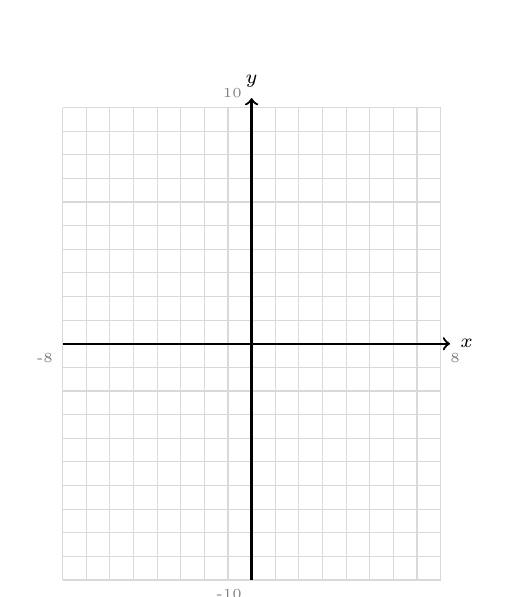
\begin{tikzpicture}[scale=0.30]
\draw[step=1,gray!30,thin] (-8,-10) grid (8,10);
\draw[->,thick] (-8,0) -- (8.4,0) node[right]{\scriptsize $x$};
\draw[->,thick] (0,-10) -- (0,10.4) node[above]{\scriptsize $y$};
\draw[gray] (-8,0) node[below left]{\tiny -8} (8,0) node[below right]{\tiny 8} (0,10) node[above left]{\tiny 10} (0,-10) node[below left]{\tiny -10};
\end{tikzpicture}}

% ---- example grid with plotted curve ----
\newcommand{\examplegrid}[5]{%
\begin{tikzpicture}[scale=0.42]
\draw[step=1,gray!30,thin] (#1,#3) grid (#2,#4);
\draw[->,thick] (#1,0) -- (#2+0.3,0) node[right]{\scriptsize $x$};
\draw[->,thick] (0,#3) -- (0,#4+0.3) node[above]{\scriptsize $y$};
\draw[brandred,very thick,domain=#1:#2,smooth,samples=80] plot (\x,{#5});
\end{tikzpicture}}

\newcommand{\quadprob}[2]{%
\begin{minipage}[t]{0.47\linewidth}
\textbf{(#1)} Graph $y = #2$.\\[1mm]
{\small Vertex: \underline{\hspace{2.1cm}} \quad Axis of sym.: \underline{\hspace{1.6cm}}\\
$x$-int.: \underline{\hspace{2.4cm}} \quad $y$-int.: \underline{\hspace{1.5cm}}\\
Opens: $\bigcirc$ Up \quad $\bigcirc$ Down}\\[2mm]
\blankgrid
\end{minipage}}

\begin{document}

% ===== Title =====
\begin{center}
  {\Huge\bfseries\color{brandred} Quadratics, Exponentials \& Sequences}\\[2mm]
  {\large\color{brandblue} A Graphing and Skills Practice Worksheet}\\[1mm]
  {\small Level: Algebra 1}\\[2mm]
  {\small \copyright\ FangMath --- All Rights Reserved}
\end{center}

\vspace{2mm}
\hrule
\vspace{3mm}

% ===================================================
\section*{Part A \ · \ Graphing Quadratic Functions}

Every quadratic function can be written in three equivalent forms. Each form makes different features easy to read directly off the equation.

\begin{center}
\renewcommand{\arraystretch}{1.5}
{\small
\begin{tabular}{|>{\raggedright\arraybackslash}p{2.6cm}|>{\raggedright\arraybackslash}p{3.1cm}|>{\raggedright\arraybackslash}p{5.4cm}|>{\raggedright\arraybackslash}p{3.4cm}|}
\hline
\rowcolor{lightblue}
\textbf{Form} & \textbf{Equation} & \textbf{What you can read directly} & \textbf{Direction / Width}\\
\hline
Standard Form & $y = ax^2 + bx + c$ & $y$-intercept $= (0,c)$; axis of symmetry $x = -\dfrac{b}{2a}$; vertex $= \left(-\dfrac{b}{2a},\, f\!\left(-\dfrac{b}{2a}\right)\right)$ & \multirow{3}{3.4cm}{$a>0$: opens up\\ $a<0$: opens down\\ $|a|>1$: narrower\\ $|a|<1$: wider}\\
\cline{1-3}
Vertex Form & $y = a(x-h)^2 + k$ & Vertex $=(h,k)$ directly; axis of symmetry $x = h$ & \\
\cline{1-3}
Intercept (Factored) Form & $y = a(x-p)(x-q)$ & $x$-intercepts $=(p,0)$ and $(q,0)$ directly; axis of symmetry $x = \dfrac{p+q}{2}$ & \\
\hline
\end{tabular}
}
\end{center}

\textit{Note: in every form, $a$ controls whether the parabola opens up or down and how narrow or wide it is.}

% ---------------------------------------------------
\subsection*{A.1 \ Standard Form: $y = ax^2+bx+c$}

\begin{examplebox}
Graph $y = x^2 - 4x + 3$.
\begin{itemize}[itemsep=1pt,topsep=2pt,leftmargin=5mm]
  \item $y$-intercept: $c = 3 \Rightarrow (0,3)$
  \item Axis of symmetry: $x = -\dfrac{b}{2a} = -\dfrac{-4}{2(1)} = 2$
  \item Vertex: $x=2 \Rightarrow y = 4-8+3=-1 \Rightarrow (2,-1)$
  \item Factor to find $x$-intercepts: $x^2-4x+3=(x-1)(x-3)=0 \Rightarrow x=1,3$
  \item $a=1>0 \Rightarrow$ opens up
\end{itemize}
\hfill
\examplegrid{-1}{5}{-2}{8}{(\x)*(\x)-4*(\x)+3}
\end{examplebox}

\begin{easybox}
\quadprob{a}{x^2-2x-3} \hfill \quadprob{b}{x^2+4x}
\end{easybox}

\begin{medbox}
\quadprob{a}{x^2-6x+5} \hfill \quadprob{b}{2x^2+4x-6}
\end{medbox}

\begin{hardbox}
\quadprob{a}{-x^2+2x+8} \hfill \quadprob{b}{2x^2-8x+3 \; \text{\small(use the vertex/quadratic formula --- roots are irrational)}}
\end{hardbox}

\newpage
% ---------------------------------------------------
\subsection*{A.2 \ Vertex Form: $y = a(x-h)^2+k$}

\begin{examplebox}
Graph $y = (x-3)^2 - 4$.
\begin{itemize}[itemsep=1pt,topsep=2pt,leftmargin=5mm]
  \item Vertex: $(h,k) = (3,-4)$ read directly
  \item Axis of symmetry: $x = 3$
  \item $y$-intercept: $x=0 \Rightarrow y=(0-3)^2-4 = 5 \Rightarrow (0,5)$
  \item $x$-intercepts: $(x-3)^2-4=0 \Rightarrow (x-3)^2=4 \Rightarrow x-3=\pm 2 \Rightarrow x=1,5$
  \item $a=1>0 \Rightarrow$ opens up
\end{itemize}
\hfill
\examplegrid{-1}{7}{-5}{6}{(\x-3)*(\x-3)-4}
\end{examplebox}

\begin{easybox}
\quadprob{a}{(x-2)^2+1 \; \text{\small(hint: no real $x$-intercepts)}} \hfill \quadprob{b}{(x+1)^2-4}
\end{easybox}

\begin{medbox}
\quadprob{a}{-2(x-1)^2+8} \hfill \quadprob{b}{\tfrac12(x+3)^2-2}
\end{medbox}

\begin{hardbox}
\quadprob{a}{-3(x+2)^2+5 \; \text{\small($x$-int.\ irrational)}} \hfill \quadprob{b}{2(x-1)^2-7 \; \text{\small($x$-int.\ irrational)}}
\end{hardbox}

\newpage
% ---------------------------------------------------
\subsection*{A.3 \ Intercept (Factored) Form: $y = a(x-p)(x-q)$}

\begin{examplebox}
Graph $y = (x-1)(x-5)$.
\begin{itemize}[itemsep=1pt,topsep=2pt,leftmargin=5mm]
  \item $x$-intercepts: $x=1$ and $x=5$ read directly
  \item Axis of symmetry: $x = \dfrac{1+5}{2} = 3$
  \item Vertex: $x=3 \Rightarrow y=(3-1)(3-5)=2(-2)=-4 \Rightarrow (3,-4)$
  \item $y$-intercept: $x=0 \Rightarrow y=(-1)(-5)=5 \Rightarrow (0,5)$
  \item $a=1>0 \Rightarrow$ opens up
\end{itemize}
\hfill
\examplegrid{-1}{7}{-5}{6}{(\x-1)*(\x-5)}
\end{examplebox}

\begin{easybox}
\quadprob{a}{(x-2)(x-4)} \hfill \quadprob{b}{(x+1)(x-3)}
\end{easybox}

\begin{medbox}
\quadprob{a}{-(x+2)(x-4)} \hfill \quadprob{b}{2(x-1)(x+3)}
\end{medbox}

\begin{hardbox}
\quadprob{a}{-2(x+3)(x-1)} \hfill \quadprob{b}{\tfrac12(x-6)(x+2)}
\end{hardbox}

\newpage
% ===================================================
\section*{Part B \ · \ Exponential Functions --- Domain and Range}

An exponential function has the form $f(x) = a\cdot b^{x-h} + k$, where $b>0$, $b\neq 1$. Transformations shift the graph but never change its basic shape.

\begin{notebox}
\textbf{Domain:} always all real numbers, $(-\infty,\infty)$, for every exponential function of this form --- there is no restriction on $x$.\\[1mm]
\textbf{Range:} determined by the horizontal asymptote $y=k$ and the sign of $a$:
\begin{itemize}[itemsep=1pt,topsep=2pt,leftmargin=5mm]
  \item If $a>0$: range is $y>k$
  \item If $a<0$: range is $y<k$
\end{itemize}
\end{notebox}

\begin{examplebox}
Find the domain and range of $f(x) = 3^x + 2$.
\begin{itemize}[itemsep=1pt,topsep=2pt,leftmargin=5mm]
  \item Domain: all real numbers, $(-\infty,\infty)$
  \item Horizontal asymptote: $y=2$; since $a=1>0$, the graph lies above the asymptote
  \item Range: $y>2$, i.e.\ $(2,\infty)$
\end{itemize}
\end{examplebox}

\begin{hardbox}
Find the domain and range of each function.

\textbf{(a)} $f(x) = -2^x - 3$

\vspace{4mm}
\textbf{(b)} $f(x) = 5\left(\dfrac{1}{2}\right)^{x-1} + 4$

\vspace{4mm}
\textbf{(c)} $f(x) = -3\cdot 2^{x+2} - 1$

\vspace{4mm}
\end{hardbox}

% ===================================================
\newpage
\section*{Part C \ · \ Arithmetic and Geometric Sequences}

\begin{notebox}
\textbf{Arithmetic sequence:} each term changes by adding a constant \textbf{common difference} $d$.
$$a_n = a_1 + (n-1)d$$
\textbf{Geometric sequence:} each term changes by multiplying by a constant \textbf{common ratio} $r$.
$$a_n = a_1 \cdot r^{\,n-1}$$
\end{notebox}

\begin{examplebox}
\textbf{Arithmetic:} Find $a_{10}$ of $5, 9, 13, 17, \dots$

$a_1=5$, $d=4 \Rightarrow a_{10} = 5+(10-1)(4) = 5+36 = 41$

\vspace{2mm}
\textbf{Geometric:} Find $a_8$ of $3, 6, 12, 24, \dots$

$a_1=3$, $r=2 \Rightarrow a_8 = 3\cdot 2^{7} = 3(128) = 384$
\end{examplebox}

\begin{easybox}
\textbf{(a) Arithmetic:} Find $a_{12}$ of the sequence $4, 7, 10, 13, \dots$

\vspace{5mm}
\textbf{(b) Geometric:} Find $a_6$ of the sequence $2, 6, 18, 54, \dots$

\vspace{5mm}
\end{easybox}

\begin{medbox}
\textbf{(a) Arithmetic:} An arithmetic sequence has $a_1 = 6$ and common difference $d = 4$. Find $a_{15}$.

\vspace{5mm}
\textbf{(b) Geometric:} A geometric sequence has $a_1 = 100$ and common ratio $r = 0.5$. Find $a_5$.

\vspace{5mm}
\end{medbox}

\begin{hardbox}
\textbf{(a) Arithmetic:} In an arithmetic sequence, $a_1=-5$, $d=4$, and $a_n = 67$. Find $n$.

\vspace{5mm}
\textbf{(b) Geometric:} In a geometric sequence, $a_1=4$, $r=3$, and $a_n = 2916$. Find $n$.

\vspace{5mm}
\end{hardbox}

% ===================================================
\newpage
\section*{Answer Key}

\subsection*{Part A --- Quadratic Functions}
{\small
\textbf{Standard Form Example:} $y=x^2-4x+3$: vertex $(2,-1)$, axis $x=2$, $x$-int.\ $1,3$, $y$-int.\ $3$, opens up.\\[1mm]
\textbf{Easy:} (a) $y=x^2-2x-3$: vertex $(1,-4)$, axis $x=1$, $x$-int.\ $-1,3$, $y$-int.\ $-3$, opens up.
\quad (b) $y=x^2+4x$: vertex $(-2,-4)$, axis $x=-2$, $x$-int.\ $0,-4$, $y$-int.\ $0$, opens up.\\[1mm]
\textbf{Medium:} (a) $y=x^2-6x+5$: vertex $(3,-4)$, axis $x=3$, $x$-int.\ $1,5$, $y$-int.\ $5$, opens up.
\quad (b) $y=2x^2+4x-6$: vertex $(-1,-8)$, axis $x=-1$, $x$-int.\ $-3,1$, $y$-int.\ $-6$, opens up.\\[1mm]
\textbf{Hard:} (a) $y=-x^2+2x+8$: vertex $(1,9)$, axis $x=1$, $x$-int.\ $4,-2$, $y$-int.\ $8$, opens down.
\quad (b) $y=2x^2-8x+3$: vertex $(2,-5)$, axis $x=2$, $x$-int.\ $x=2\pm\frac{\sqrt{10}}{2}\approx 3.58, 0.42$, $y$-int.\ $3$, opens up.\\[3mm]

\textbf{Vertex Form Example:} $y=(x-3)^2-4$: vertex $(3,-4)$, axis $x=3$, $x$-int.\ $1,5$, $y$-int.\ $5$, opens up.\\[1mm]
\textbf{Easy:} (a) $y=(x-2)^2+1$: vertex $(2,1)$, axis $x=2$, no real $x$-int., $y$-int.\ $5$, opens up.
\quad (b) $y=(x+1)^2-4$: vertex $(-1,-4)$, axis $x=-1$, $x$-int.\ $1,-3$, $y$-int.\ $-3$, opens up.\\[1mm]
\textbf{Medium:} (a) $y=-2(x-1)^2+8$: vertex $(1,8)$, axis $x=1$, $x$-int.\ $3,-1$, $y$-int.\ $6$, opens down.
\quad (b) $y=\tfrac12(x+3)^2-2$: vertex $(-3,-2)$, axis $x=-3$, $x$-int.\ $-1,-5$, $y$-int.\ $2.5$, opens up.\\[1mm]
\textbf{Hard:} (a) $y=-3(x+2)^2+5$: vertex $(-2,5)$, axis $x=-2$, $x$-int.\ $x=-2\pm\sqrt{5/3}\approx-0.71,-3.29$, $y$-int.\ $-7$, opens down.
\quad (b) $y=2(x-1)^2-7$: vertex $(1,-7)$, axis $x=1$, $x$-int.\ $x=1\pm\sqrt{3.5}\approx2.87,-0.87$, $y$-int.\ $-5$, opens up.\\[3mm]

\textbf{Intercept Form Example:} $y=(x-1)(x-5)$: vertex $(3,-4)$, axis $x=3$, $x$-int.\ $1,5$, $y$-int.\ $5$, opens up.\\[1mm]
\textbf{Easy:} (a) $y=(x-2)(x-4)$: vertex $(3,-1)$, axis $x=3$, $x$-int.\ $2,4$, $y$-int.\ $8$, opens up.
\quad (b) $y=(x+1)(x-3)$: vertex $(1,-4)$, axis $x=1$, $x$-int.\ $-1,3$, $y$-int.\ $-3$, opens up.\\[1mm]
\textbf{Medium:} (a) $y=-(x+2)(x-4)$: vertex $(1,9)$, axis $x=1$, $x$-int.\ $-2,4$, $y$-int.\ $8$, opens down.
\quad (b) $y=2(x-1)(x+3)$: vertex $(-1,-8)$, axis $x=-1$, $x$-int.\ $1,-3$, $y$-int.\ $-6$, opens up.\\[1mm]
\textbf{Hard:} (a) $y=-2(x+3)(x-1)$: vertex $(-1,8)$, axis $x=-1$, $x$-int.\ $-3,1$, $y$-int.\ $6$, opens down.
\quad (b) $y=\tfrac12(x-6)(x+2)$: vertex $(2,-8)$, axis $x=2$, $x$-int.\ $6,-2$, $y$-int.\ $-6$, opens up.
}

\subsection*{Part B --- Exponential Domain \& Range}
{\small
\textbf{Example:} $f(x)=3^x+2$: domain $(-\infty,\infty)$, range $y>2$.\\[1mm]
\textbf{(a)} $f(x)=-2^x-3$: domain $(-\infty,\infty)$; asymptote $y=-3$, $a=-1<0$, range $y<-3$.\\
\textbf{(b)} $f(x)=5(\tfrac12)^{x-1}+4$: domain $(-\infty,\infty)$; asymptote $y=4$, $a=5>0$, range $y>4$.\\
\textbf{(c)} $f(x)=-3\cdot2^{x+2}-1$: domain $(-\infty,\infty)$; asymptote $y=-1$, $a=-3<0$, range $y<-1$.
}

\subsection*{Part C --- Arithmetic \& Geometric Sequences}
{\small
\textbf{Example:} Arithmetic $a_{10}=41$. \quad Geometric $a_8=384$.\\[1mm]
\textbf{Easy:} (a) $a_{12}=4+(11)(3)=37$. \quad (b) $a_6=2\cdot3^5=486$.\\
\textbf{Medium:} (a) $a_{15}=6+(14)(4)=62$. \quad (b) $a_5=100(0.5)^4=6.25$.\\
\textbf{Hard:} (a) $67=-5+(n-1)(4) \Rightarrow n=19$. \quad (b) $2916=4\cdot3^{\,n-1} \Rightarrow 3^{\,n-1}=729=3^6 \Rightarrow n=7$.
}

\vspace{4mm}
\hrule
\vspace{2mm}
\begin{center}
{\small \copyright\ FangMath --- All Rights Reserved. Not to be reproduced or distributed without permission.}
\end{center}

\end{document}
